\begin{figure}
\setlength{\unitlength}{\textwidth}

  \begin{picture}(1,0.35)(0,0.75)
    
  \put(0.15,0.76){\includegraphics[width=0.7\unitlength]{../FnP/gnuplot/mean_power_collapsed_mstar.eps}}         
      
      
   
 	\put(0.11,0.95){\large $\frac{P_{m}}{\rho \mathcal{A}U^3 }$} 	

 	
 	 	\put(0.45,0.75){ $c\rho\mathcal{A}U$} 	
 	 

     

  \end{picture}

  \caption{Mean power as a function of damping factor. Data are presented at $m^*=10$ (\ding{108}), $m^*=20$ (\ding{83}), $m^*=40$ (\ding{115}), $m^*=60$ (+) at Re 165 and $\zeta=0.1$. A reduction of maximum mean power can be observed when $m^*<40$. For $m^*>40$, the maximum power is essentially independent of $m^*$.}
    \label{fig:m_star_collapsed}
\end{figure}